\subsubsection{Purpose}
Another great feature of Travlendar+, besides the capability of displaying into the user's events schedule which kind of transport means the user should take to reach the location of each appointments, he/she can take public transportation by buying tickets directly within the application or by inserting his pass code. If a user should take a taxi, he can easily book it by calling the local taxi service company. The application, after locating a shared transport of a vehicle sharing system, such as a bike or car, will allow the user to pay with his credit card from the application.

\subsubsection{Scenario 1}
Alice is a 22-year-old student and she uses Travlendar+ to organize university courses between campus Bovisa and campus Leonardo. Alice does not use the car and among the system setting she has set public transport as means of transportation. Travlendar+ will suggest Alice to use either public transport (including taxi service) or vehicle sharing services. After entering all the lecture of the day, Travlendar+ advises Alice the meter as means of transport to take between lessons at Campus Bovisa and lessons at Campus Leonardo.
Alice, by simply accessing the general information of the event, will be able to buy a metro ticket through the local public transport application.
Once she has purchased the ticket, in general information of the event, Travlendar+ shows to Alice the QR code, which will allow her to take the subway in order to make the desired transfer.

\subsubsection{Scenario 2}
Bob is a personal trainer who lives in Milan, and wants to organize his fitness courses through Travlendar+ application.
After registering and setting general preferences for the means of transport to be use, Bob adds a course he will have to do in the afternoon. The application automatically calculates every possible route and shows him the fastest, which must be run with the bicycle. Unfortunately, Bob does not have a bike available at this time, so he does not know how to reach the location.
However, Travlendar+ incorporates a feature that allows the user to use local bike sharing services simply by accessing through the general information interface of the event.
Bob, by clicking on the bike sharing service (e.g. Mobike), can locate the bikes closest to him and takes the one that is most comfortable in order to reaching the destination as fast as possible.

\subsubsection{Use case}
The use case diagram for mobility selection is shown in Figure \ref{fig:useCaseMobility}, whereas the use case diagram for purchasing tickets is shown in Table \ref{usecase_tickets}.
\begin{figure}
	\centering
	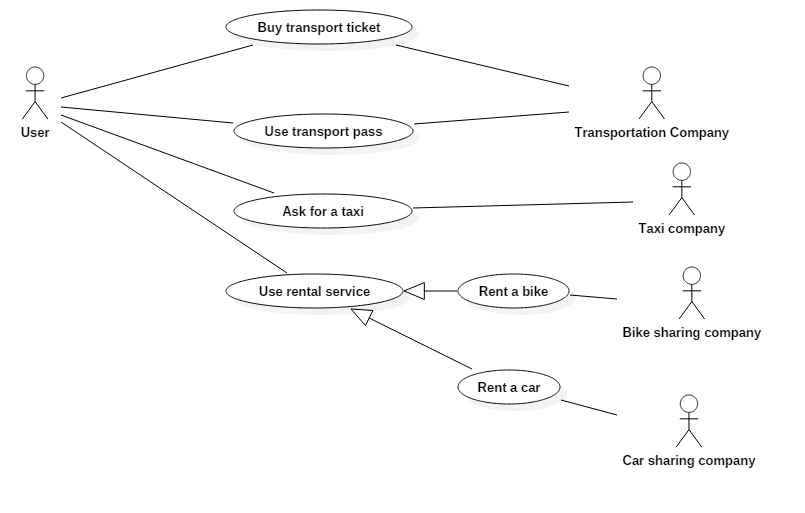
\includegraphics[width=6in]{./diagrams/TransportationUseCase.png}
	\caption{Use case diagram for mobility selection}
	\label{fig:useCaseMobility}
\end{figure}

\begin{table}
\centering
	\begin{tabular}{|c||p{0.6\textwidth}|}
    \hline
    Name & Purchase Tickets \\ \hline
    Actors & User \\  \hline
    Input condition & The user has already added at least one appointment and has been validated \\ \hline
    Flow of events & \begin{enumerate}
    \item The user may want to buy a public transport ticket
    \item The system forward the request to an external service in order to process the data and check the availability of the ticket.
    \item The external transport company API checks if there are tickets which are still purchased and asks to user the confirmation of buy the ticket.
    \end{enumerate} \\ \hline
     Output condition & The QR code of the tickets that he has purchased are added into the specific windows where the user can manage all his public transport ticket. \\ \hline
     Exception & The ticket may not be available for a specific means of transport (metro, bus, tram) \\ \hline
	\end{tabular}
\caption{Use case for purchasing tickets}
\label{usecase_tickets}
\end{table}

\subsubsection{Sequence diagram}
The sequence diagram of the purchase tickets process is illustrated in Figure \ref{fig:seqPurchaseTickets}, whereas the sequence diagram of the vehicle sharing process is illustrated in Figure \ref{fig:seqVehicleSharing}.
\begin{figure}
	\centering
	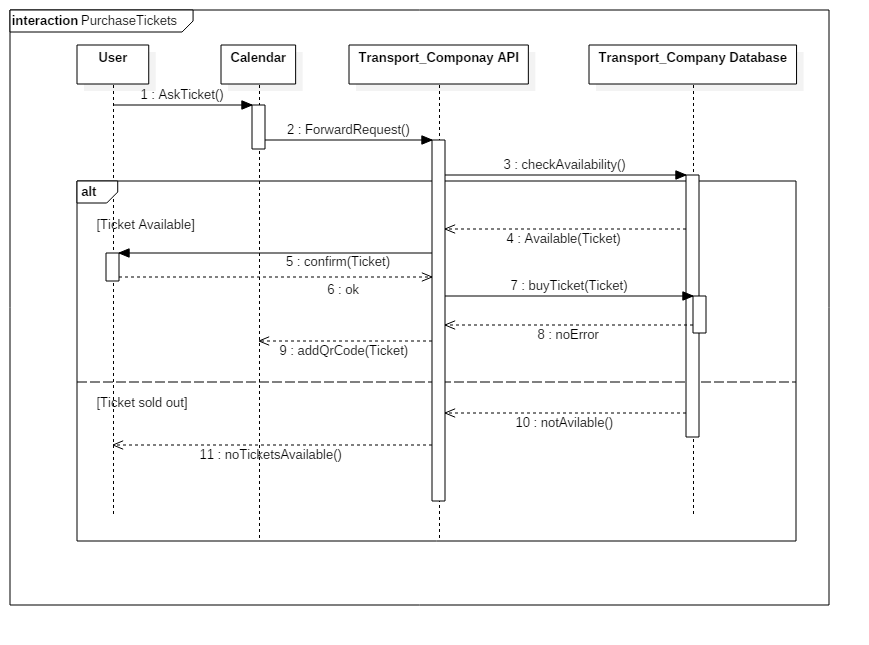
\includegraphics[width=6in]{./diagrams/PurchaseTickets.png}
	\caption{Sequence diagram: Purchase Tickets}
	\label{fig:seqPurchaseTickets}
\end{figure}

\begin{figure}
	\centering
    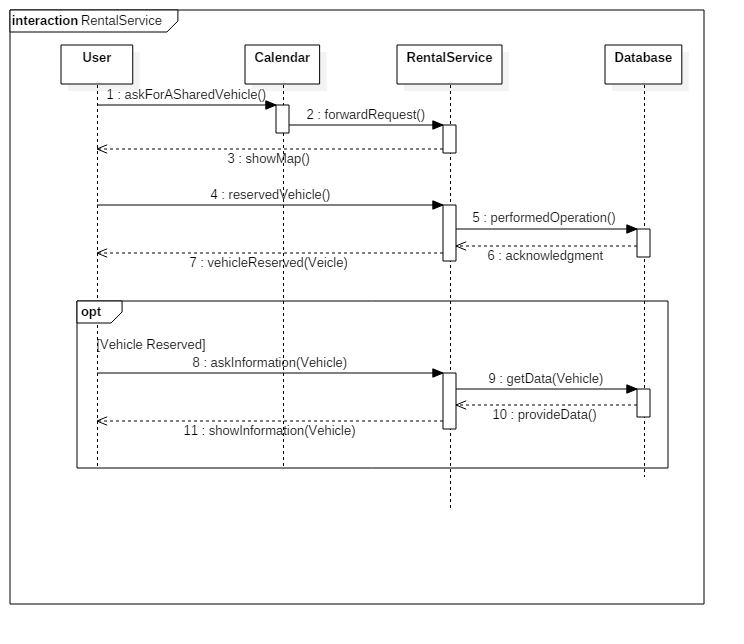
\includegraphics[width=6in]{./diagrams/RentalService.png}
    \caption{Sequence diagram: Vehicle Sharing}
    \label{fig:seqVehicleSharing}
\end{figure}

\subsubsection{Associated functional requirements}
\begin{enumerate}
\item The system offers the possibility to buy public transportation tickets when a bus, a metro or a tram should be taken.
\item The user can add his personal day/week/season pass when he has to take public transportation.
\begin{itemize}
\item When a user has to take a public transport he can type in his pass code. The system automatically checks the pass code by forwarding the request to the local public transportation API.
\end{itemize}
\item The system displays all the possible vehicle sharing system in the general information interface of the event, if it should be taken. In particular the two ones are:
		\begin{itemize}
        \item Car sharing system (e.g. Enjoy, Car2go)
        \item Bike sharing system (e.g Mobike)
		\end{itemize}
\item The system allows the user to locate the vehicle available around him, by accessing to the map that the application provides.
\begin{itemize}
\item When the user has to take a car, he can reserve it and access to all the information that he needs through the application.
\item When the user has to take a bike, he can locate it through the map and take it through the specific sharing service API.
\end{itemize}
\item The system includes a taxi service, that allows user to reserve a taxi by calling the local taxi service with the number that the application shows to him.
\end{enumerate}

\subsubsection{Mockups}
The mockup of the ticket purchase is shown in Figure \ref{fig:seqPurchaseTicket}.
\begin{figure}
	\centering
    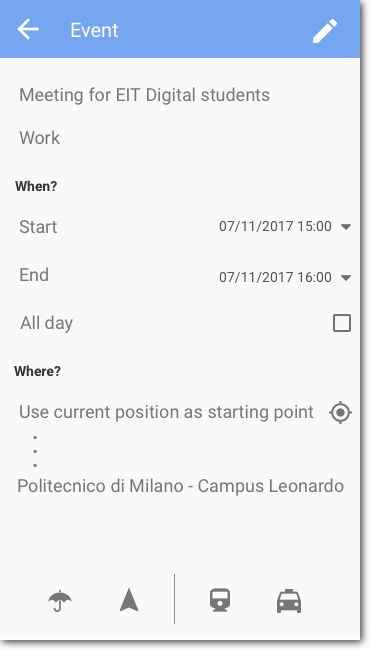
\includegraphics[width=4.5in]{./images/event.png}
    \caption{Purchase ticket mockup.}
    \label{fig:seqPurchaseTicket}
\end{figure}